\documentclass[12pt,a4paper]{article}

\usepackage[T1]{fontenc}
\usepackage[utf8]{inputenc}
\usepackage[margin=2.5cm]{geometry}
\usepackage{graphicx}
\usepackage{subcaption}
\usepackage[hidelinks]{hyperref}
\usepackage{fancyhdr}
\usepackage{lastpage}
\usepackage{appendix}
\usepackage{mdframed}
\usepackage{color}
\usepackage{palatino}
\usepackage{mathtools}
\usepackage{changepage}
\usepackage{subcaption}
\usepackage{enumitem}
\usepackage{csquotes}
\usepackage{verbatim}
\usepackage[cache=false]{minted}
\usepackage[ruled,vlined]{algorithm2e}

\DeclarePairedDelimiter{\ceil}{\lceil}{\rceil}
\DeclarePairedDelimiter\floor{\lfloor}{\rfloor}

\usemintedstyle{default}
\setminted{
  linenos=true,
  breaklines=true,
  fontsize=\small,
  frame=single,
}

\title{Lazy Selection}
\author{Carlos Requena López}

%% Fancy layout
\pagestyle{fancy}
\lhead{Lazy selection}
\chead{}
\rhead{}
\lfoot{}
\cfoot{}
\rfoot{Page \thepage\ of \pageref{LastPage}}
\renewcommand{\headrulewidth}{0.4pt}
\renewcommand{\footrulewidth}{0.4pt}

\newtheorem{theorem}{Theorem}


%%% --- %%% --- DOCUMENT START --- %%% --- %%%
\begin{document}
\maketitle
\pagestyle{fancy}

\section{Introduction}

This assignment tries to empirically verify Theorem 3.5 (here
\ref{theo1}) from \cite[p.~49]{motwani}, running the
\textbf{LazySelect} algorithm for different values of $n$ and $k$ to
establish the asymptotic behaviour of the number of comparisons
performed.

The \textbf{LazySelect} algorithm finds the $k$th smallest element in
a set $S$ (assumed to have total order) of size $n$. It essentially
outputs the element with rank $k$. Concerning notation, $A_{(i)}$ will
refer to the element with rank $i$ in set $A$ and $r_A(j)$ will refer
to the rank of element $j$ in set $A$.
\section{Analysis and expectations}

We detail the steps of the aforementioned algorithm in Algorithm
\ref{algo:lazyselect}.

\begin{algorithm}[h]
  \SetAlgoLined
  \KwIn{An (unsorted) array $S$ of size $n$ and and integer $k < n$}
  \KwOut{The element in $S$ that has rank $k$}

  \nl Take a random sample of $n^{3/4}$ elements of S. Call it $R$\;
  \nl Sort R\;
  \nl Define $x = kn^{-1/4}$. With $\ell = \text{max}\{\floor{x -
    \sqrt{n}}, 1\}$ and $h = \text{min}\{\ceil{x - \sqrt{n}\ \ }, n^{3/4}\}$\;
  \nl Assign $a = R_{(\ell)}$ and $b = R_{(h)}$\;
  \nl Determine the rank of $a$ and $b$ in $S$. That is, find $r_{S}(a)$
  and $r_{S}(b)$\;
  \nl \uIf{$k < n^{1/4} $}{$P = \{y \in S\ |\ y \leq b\}$}
  \uElseIf{$k > n - n^{1/4}$}{$P = \{y \in S\ |\ y \geq a\}$}
  \ElseIf{$k \in [n^{1/4}\, n - n^{1/4}]$}{$P = \{y \in S\ |\ a \leq y
    \leq b\}$}
  \nl Check whether $S_{(k)} \in P$ \emph{and} $|P| \leq 4n^{3/4} +
  2$. If not, repeat steps 1 through 6\;
  \nl If the conditions are satisfied: sort $P$ and look for $S_{(k)}$
  in $P$\;
  \caption{\bf LazySelect}
  \label{algo:lazyselect}
\end{algorithm}

We can make some observations about this algorithm:
\begin{itemize}
\item By taking $R$, we hope it will be a good representative of the
  original set $S$.
\item Any optimal sorting algorithm works for step 2. The number of
  comparisons performed is sublinear: $\mathcal{O}(n^{3/4}\log(n))$
\item $x$ is a sort of rank scaling. Rank $x$ is to $R$ what $k$ is to $S$
  (roughly).
\item When $k < n^{1/4}$ and $S_{(k)} \in P$, the element is simply
  $P_{(k)}$.
\item The elements are put back to simplify the analysis, since the random
  variables used become independent.
\end{itemize}

Also, as proved in \cite[p.~49]{motwani}, we have:

\begin{mdframed}
  \begin{theorem}
    With probability $1 - \mathcal{O}(n^{-1/4})$,
    \textbf{\textup{LazySelect}} finds $S_{(k)}$ on the first pass,
    and thus performs only $2n + o(n)$ comparisons.
    \label{theo1}
  \end{theorem}
\end{mdframed}

Indeed, finding the rank of $a$ and $b$ in $S$ takes linear time for
both $a$ and $b$, and the sorting or $R$ and $P$ takes sublinear time,
hence little-o of $n$.

\section[Implementation and results]{Implementation and results\footnote{Code can be found at
\url{https://github.com/carlosgeos/lazy-selection}}}

Having the version of the algorithm that reports the number of
comparisons implemented, we can run a series of test to find the
asymptotic behaviour of this number and the distribution of it, for
different values of $n$ and $k$.

For every $n$ and $k$, we run \textbf{LazySelect} a significant number
of times, starting at ten thousand times for $n = 100$ and finishing
at fifty times for $n = 10^6$. Then we build a histogram to visualise
the distribution of the number of comparisons performed.

To determine the asymptotic behaviour, we plot in a line chart the
average number of comparisons against the number of elements.


% \ref{fig:sample-input}

\begin{figure}[ht!]
  \centering
  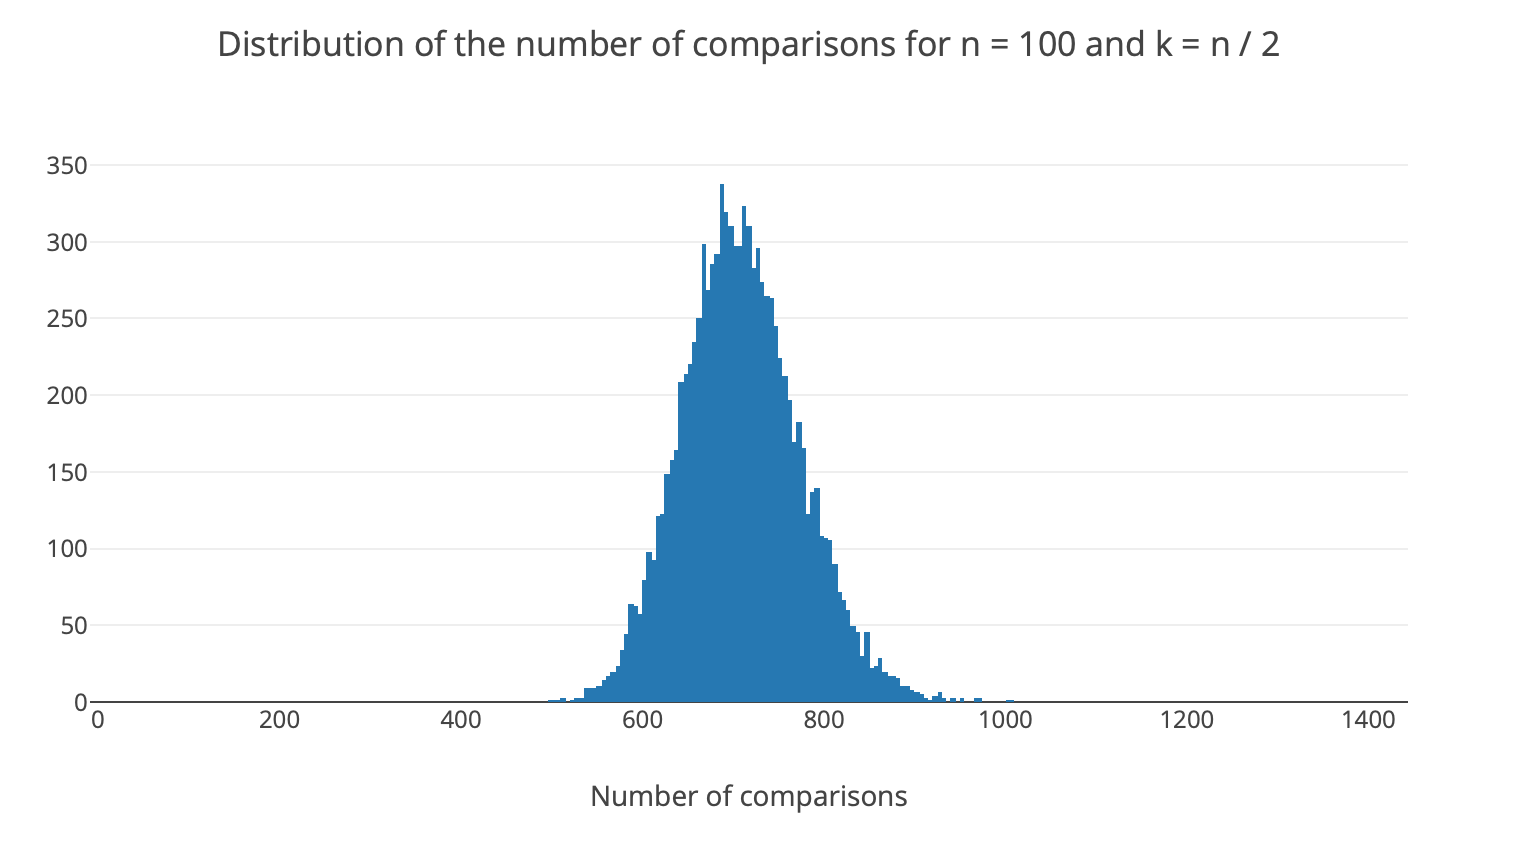
\includegraphics[width=0.9\textwidth]{img/n100k50.png}
  \caption{}
  \label{fig:}
\end{figure}

\begin{figure}[ht!]
  \centering
  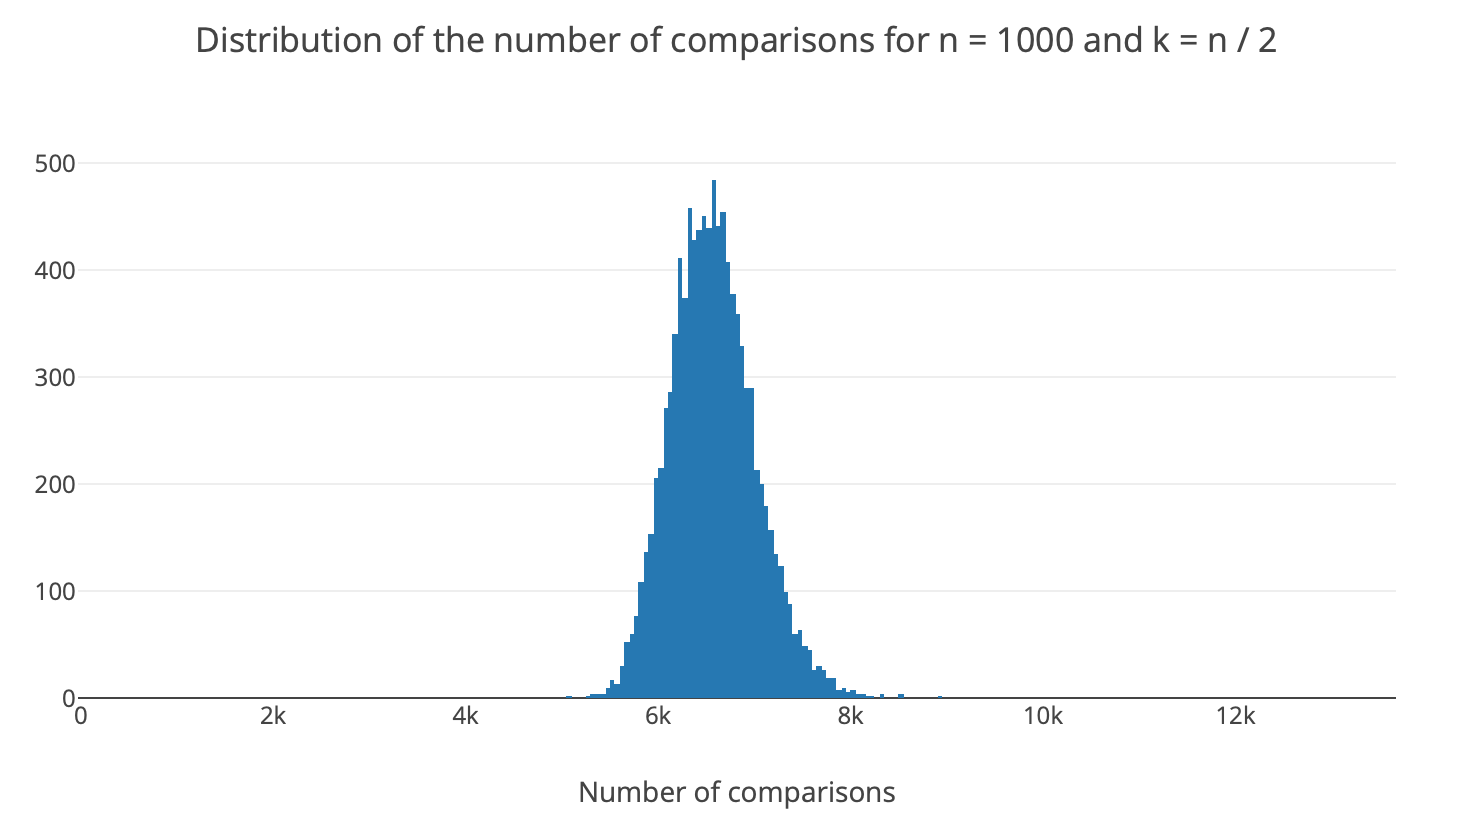
\includegraphics[width=0.9\textwidth]{img/n1000k500.png}
  \caption{}
  \label{fig:}
\end{figure}

\begin{figure}[ht!]
  \centering
  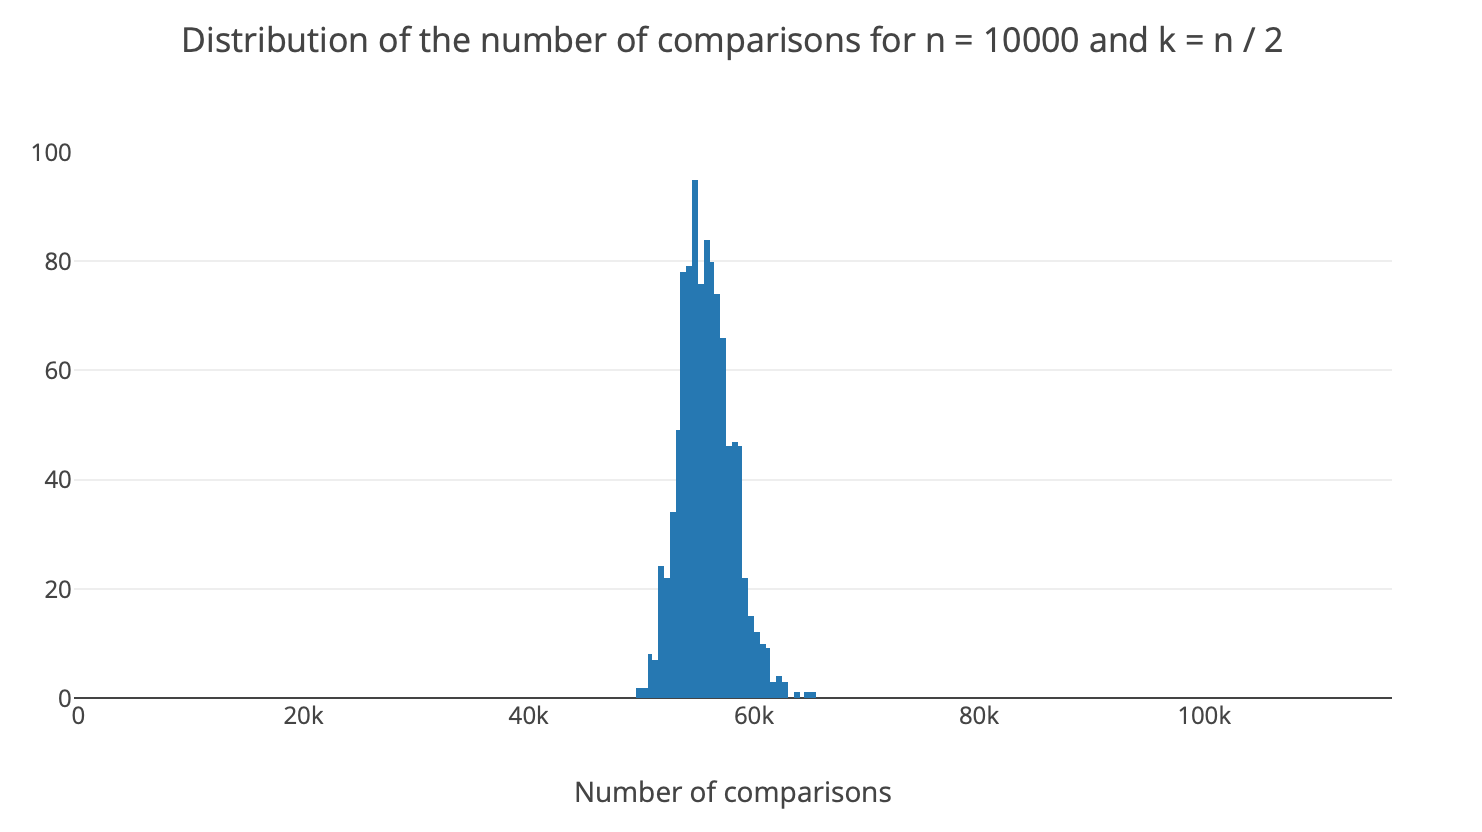
\includegraphics[width=0.9\textwidth]{img/n10000k5000.png}
  \caption{}
  \label{fig:}
\end{figure}

\begin{figure}[ht!]
  \centering
  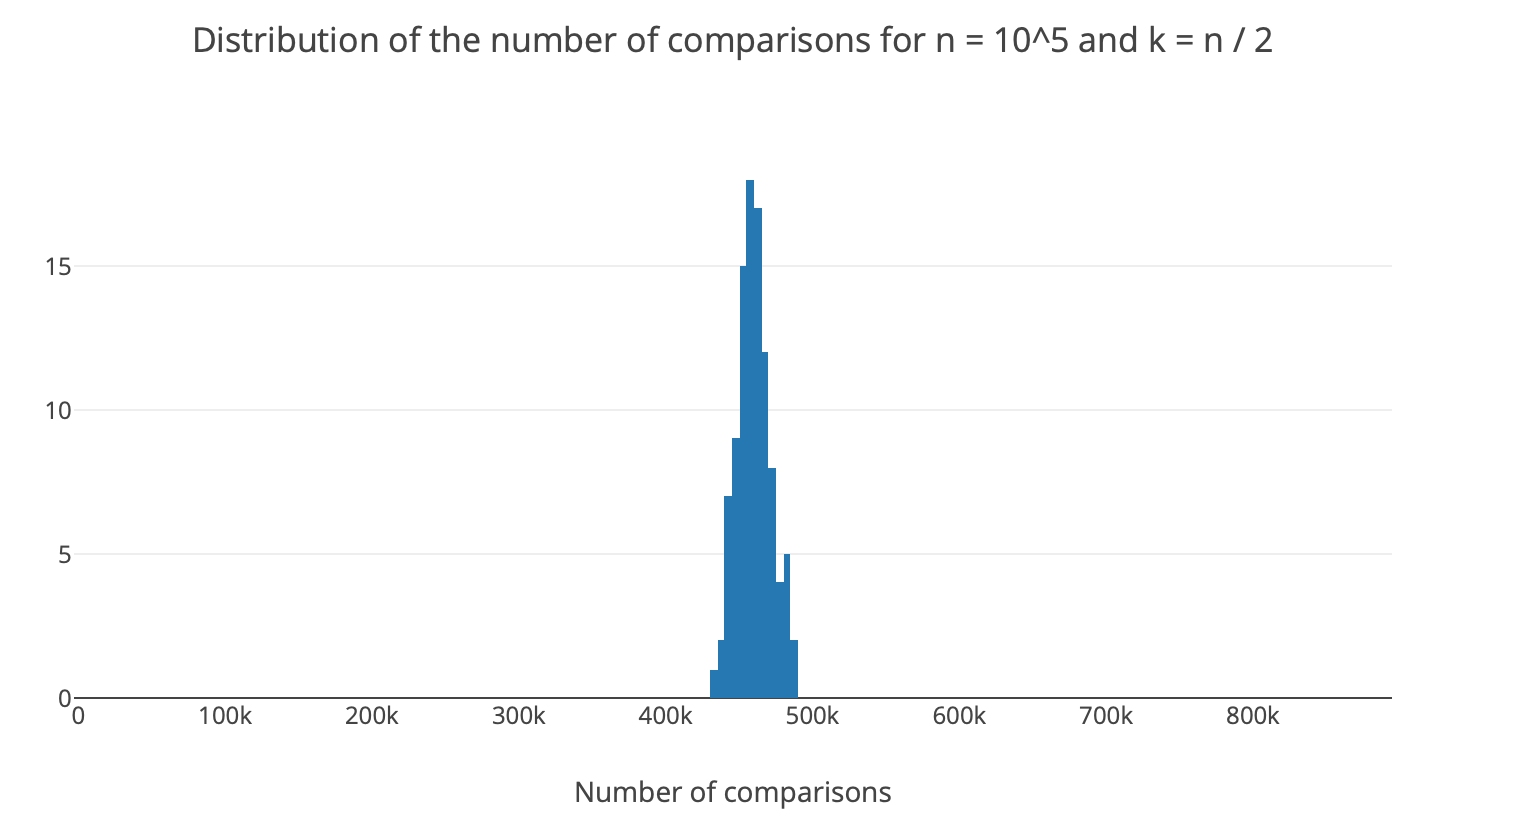
\includegraphics[width=0.9\textwidth]{img/n100000k50000.png}
  \caption{}
  \label{fig:}
\end{figure}

\begin{figure}[ht!]
  \centering
  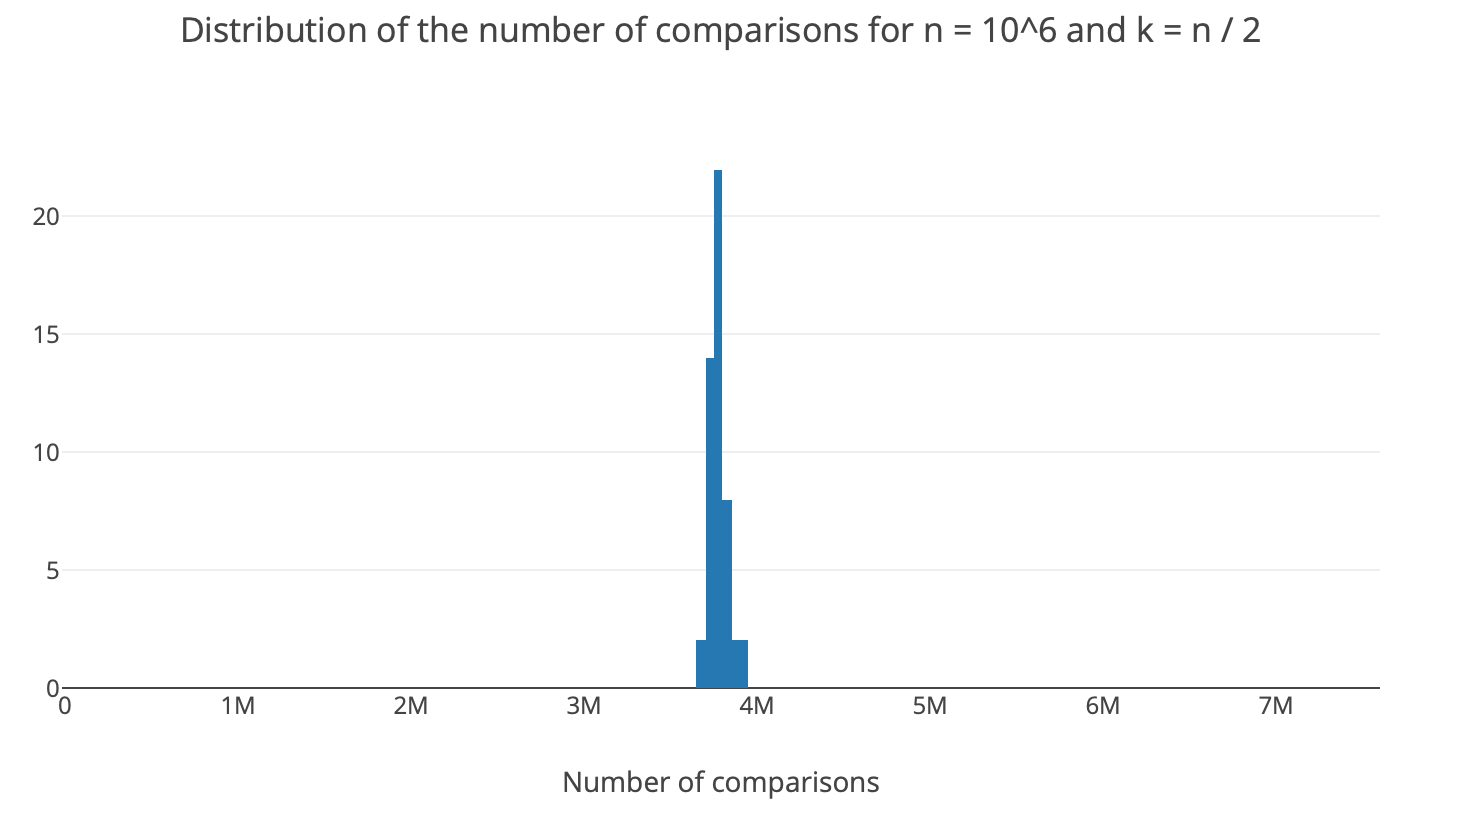
\includegraphics[width=0.9\textwidth]{img/n1000000k500000.png}
  \caption{}
  \label{fig:}
\end{figure}

\begin{figure}[ht!]
  \centering
  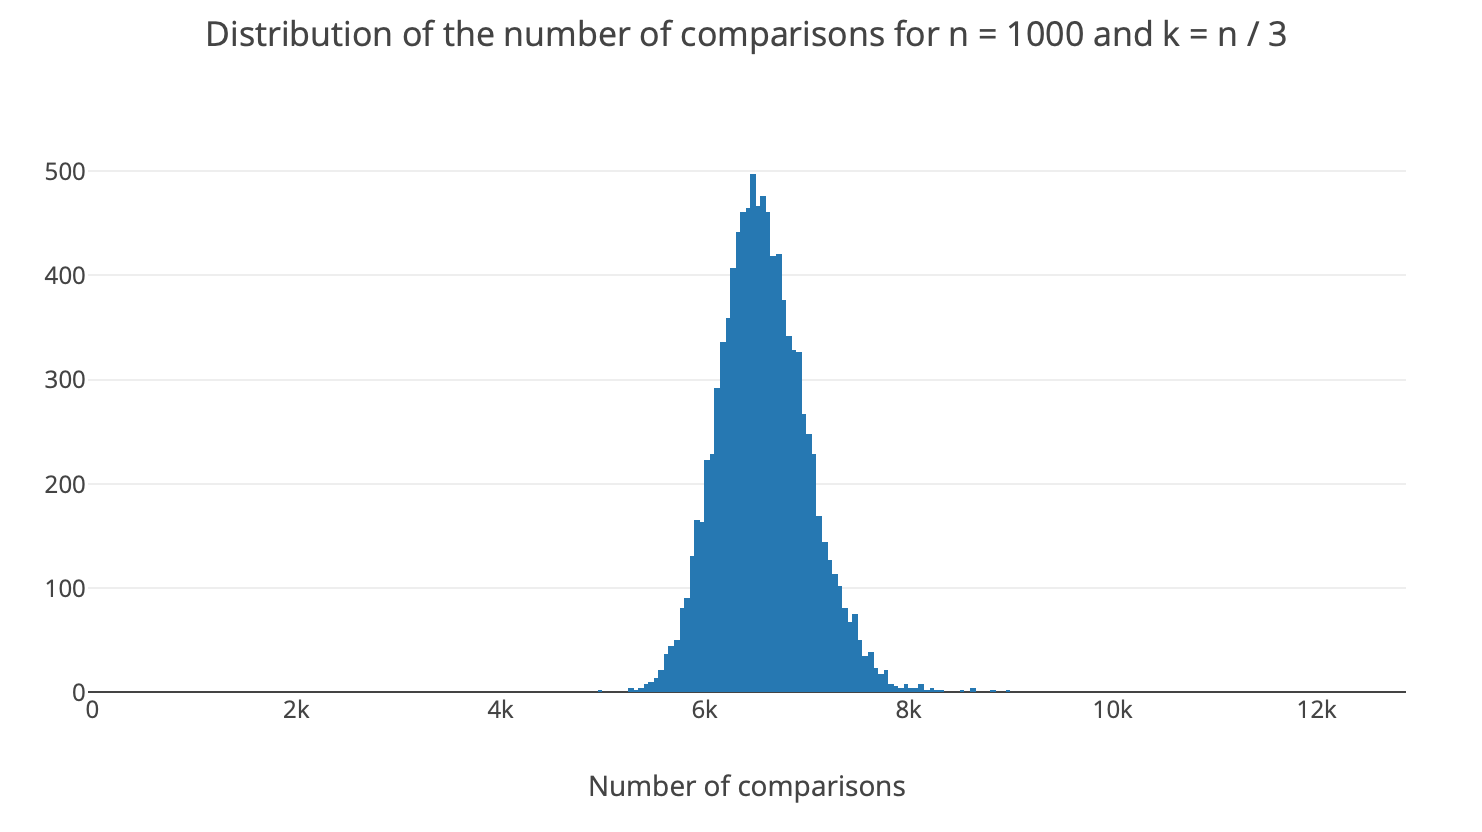
\includegraphics[width=0.9\textwidth]{img/kdiv3.png}
  \caption{}
  \label{fig:div3}
\end{figure}

\begin{figure}[ht!]
  \centering
  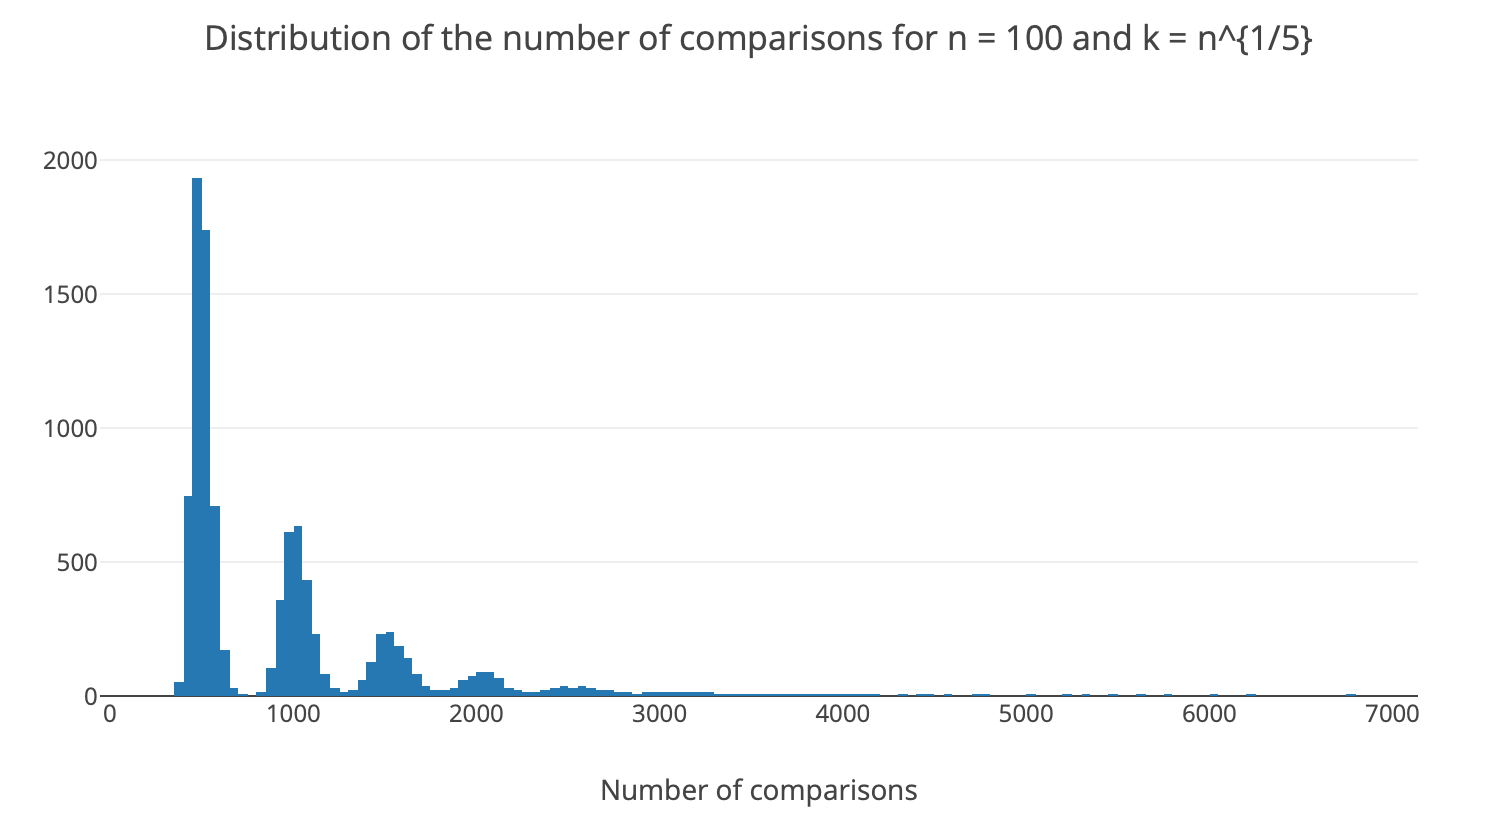
\includegraphics[width=0.9\textwidth]{img/kroot5.png}
  \caption{}
  \label{fig:root5}
\end{figure}

\begin{figure}[ht!]
  \centering
  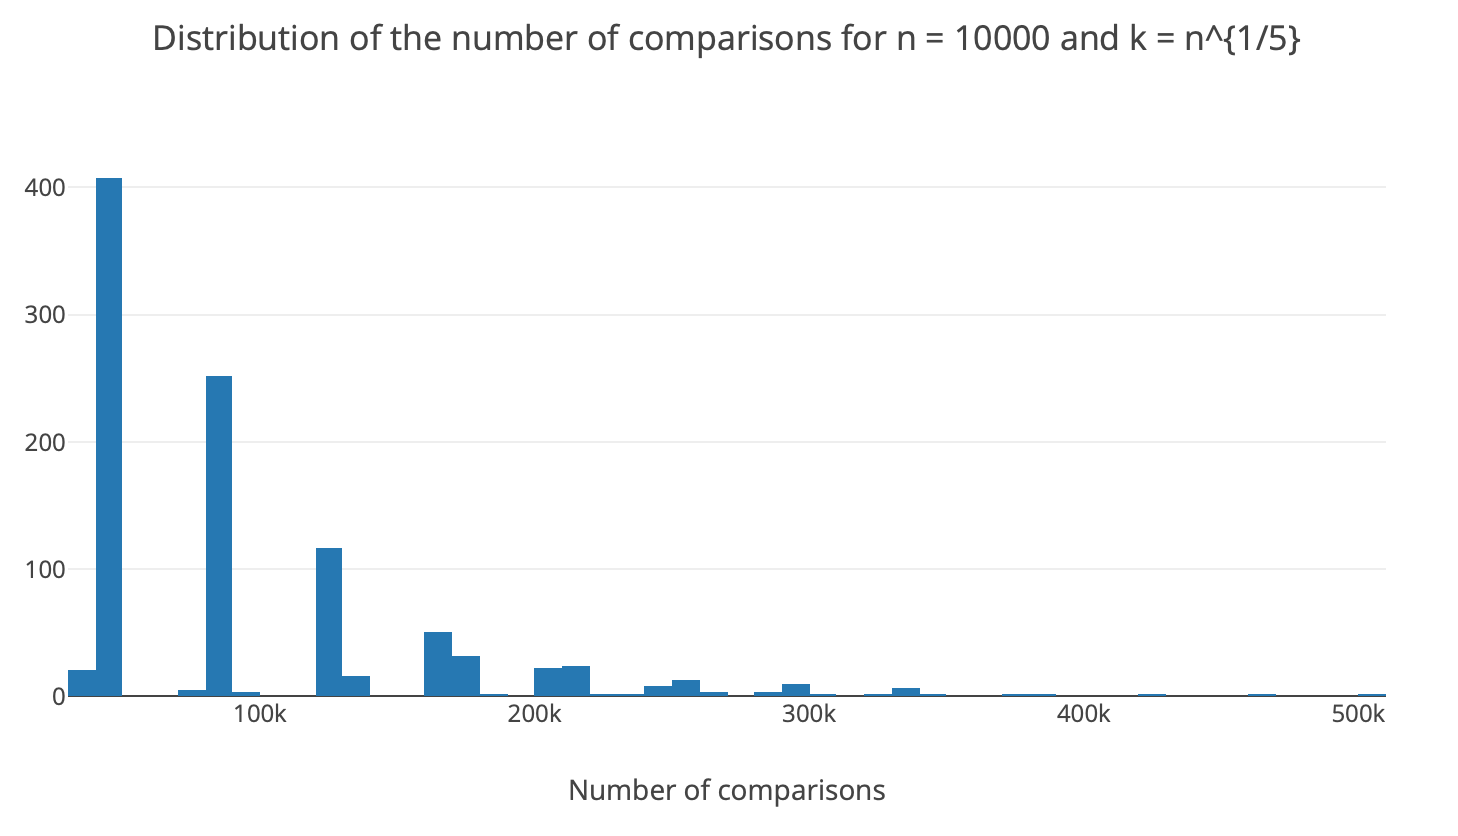
\includegraphics[width=0.9\textwidth]{img/kroot5-2.png}
  \caption{}
  \label{fig:root5-2}
\end{figure}

\begin{figure}[ht!]
  \centering
  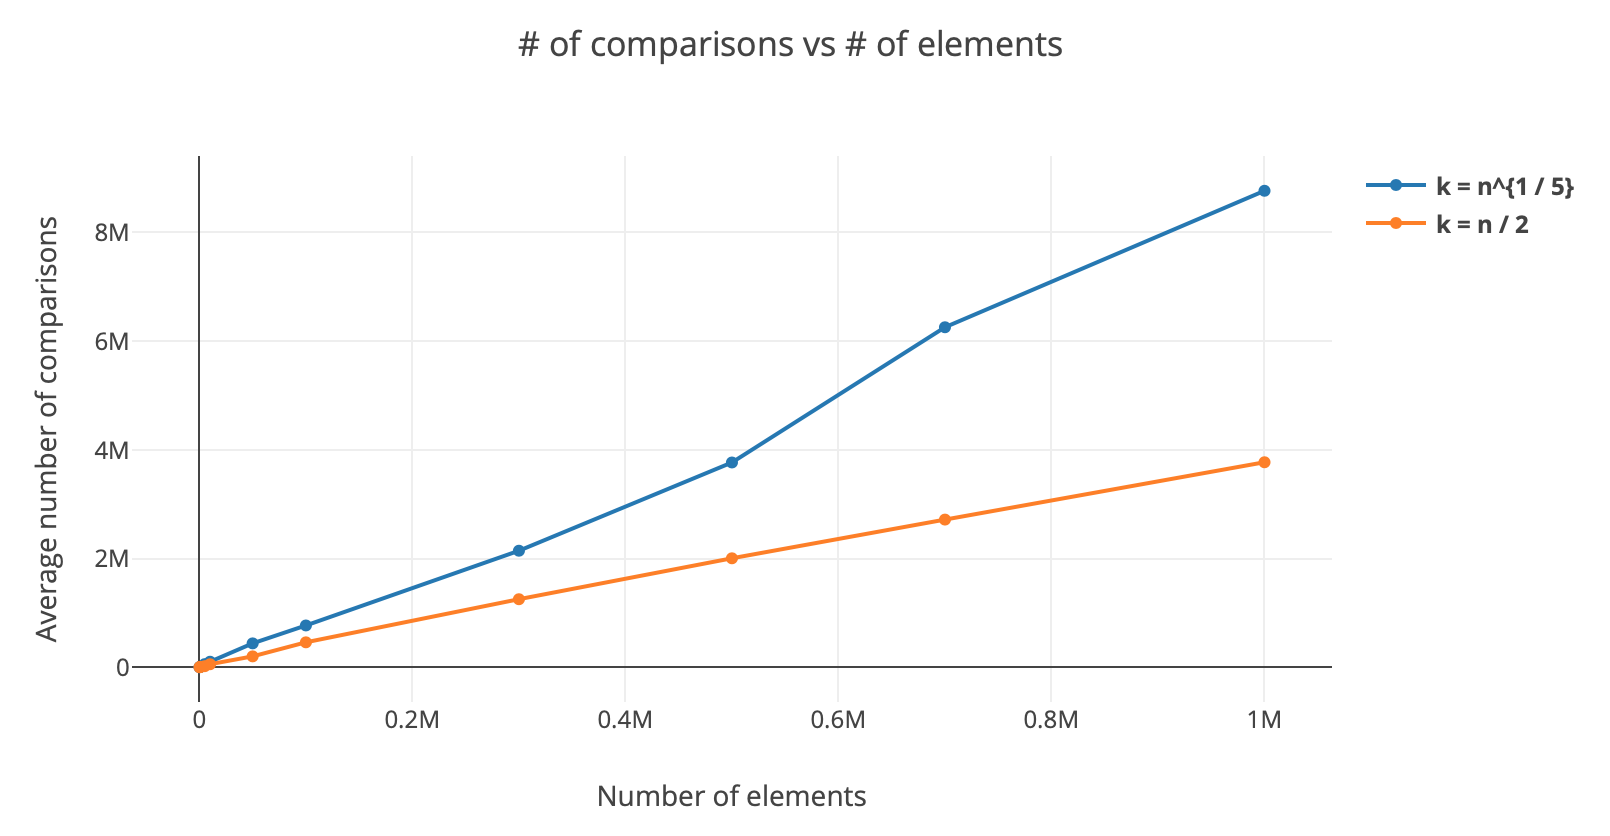
\includegraphics[width=0.9\textwidth]{img/asym.png}
  \caption{}
  \label{fig:asym}
\end{figure}

\clearpage

\section{Conclusion}

The algorithm behaves as described in Theorem 1. If $k$ is set to the
median, the histograms show how virtually all runs end up doing
$2n + o(n)$ comparisons.

An interesting feature happens in figures \ref{fig:root5} and
\ref{fig:root5-2}. They show how, if $k$ is sufficiently small or
large, the algorithm does not satisfy the two conditions and
iterates. The decreasing size clusters to the right of the first one
show the negative exponential $\mathcal{O}(n^{1/4})$ probability of
having to perform successive iterations.

Figure \ref{fig:div3} shows that for a moderate $k$, results are no
different than the ones obtained when setting $k$ to the median. The
result is the same for other $n$ (not shown).

These tests were all done with a random dataset in which all numbers
had the same probability of appearing. However, if we had a skewed
dataset, we could guess the results would be similar to those found by
tweaking $k$.

Finally, figure \ref{fig:asym} shows the linearity of the number of
comparisons as $n$ grows (both axes are linear), and the extra cost of
finding a very small or very large element in $S$.

\nocite{*}
\bibliographystyle{plain}
\bibliography{refs}


\appendix
\section{Appendix - code listing}

\inputminted[label=core.clj]{clojure}{../src/lazy_selection/core.clj}

\end{document}
